\documentclass{standalone}
\usepackage{tikz}
\usetikzlibrary{patterns, positioning}


\begin{document}
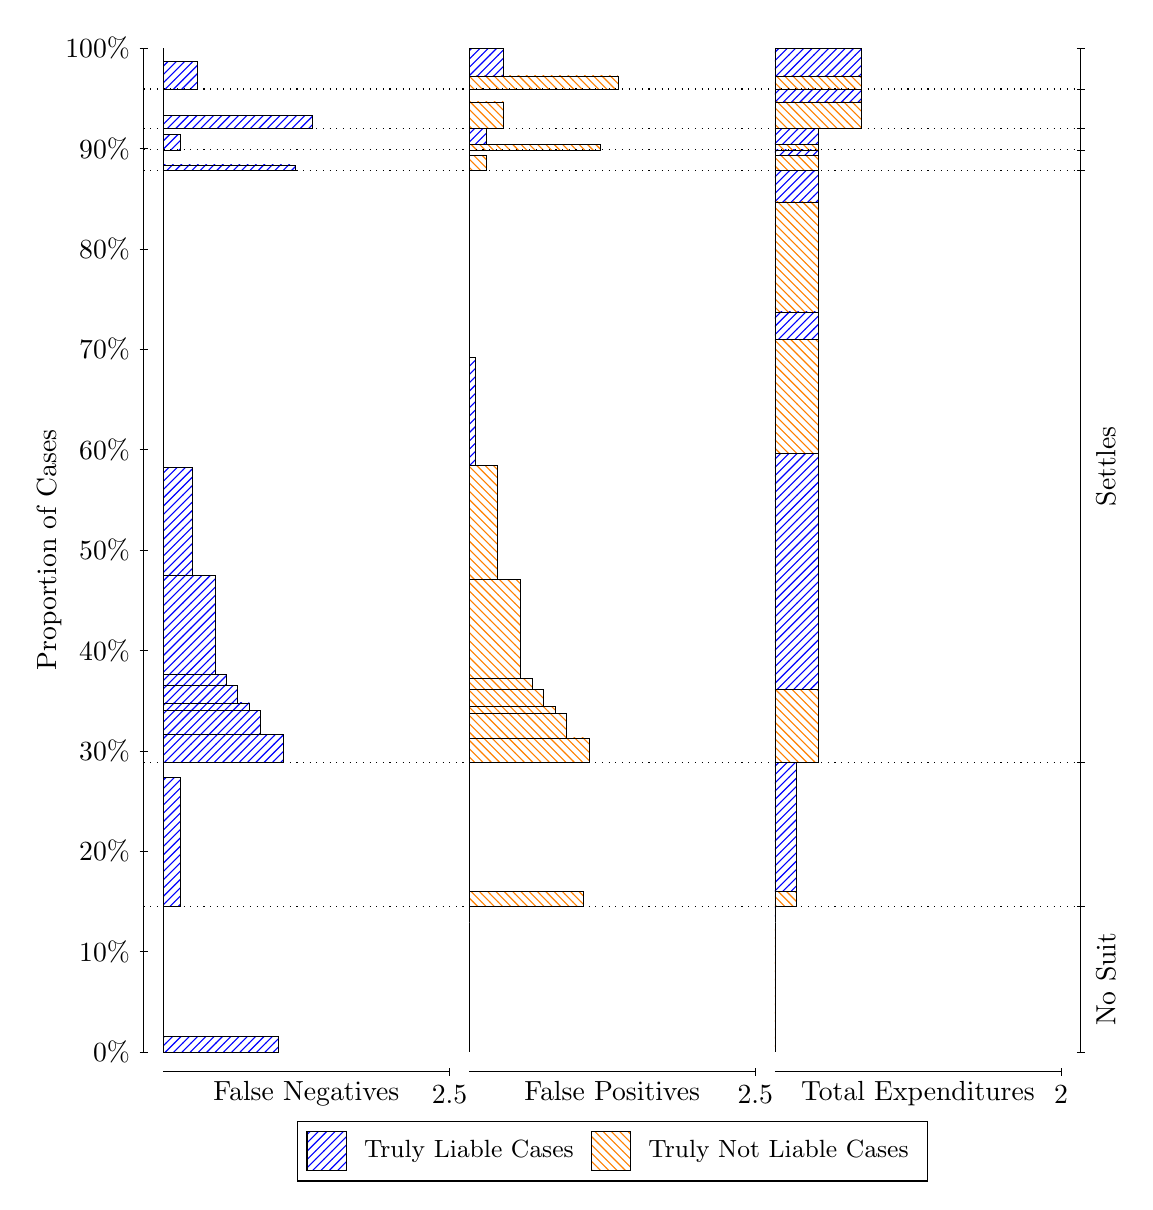
\begin{tikzpicture}
\draw[black, very thin] (1.5,1.75) -- (1.5,14.5);
\node[rotate=90, text=black, anchor=center] at (0.3, 8.125) {Proportion of Cases};
\draw[black, very thin] (1.45,1.75) -- (1.55,1.75);
\node[text=black, anchor=east] at (1.45, 1.75) {0\%};
\draw[black, very thin] (1.45,3.025) -- (1.55,3.025);
\node[text=black, anchor=east] at (1.45, 3.025) {10\%};
\draw[black, very thin] (1.45,4.3) -- (1.55,4.3);
\node[text=black, anchor=east] at (1.45, 4.3) {20\%};
\draw[black, very thin] (1.45,5.575) -- (1.55,5.575);
\node[text=black, anchor=east] at (1.45, 5.575) {30\%};
\draw[black, very thin] (1.45,6.85) -- (1.55,6.85);
\node[text=black, anchor=east] at (1.45, 6.85) {40\%};
\draw[black, very thin] (1.45,8.125) -- (1.55,8.125);
\node[text=black, anchor=east] at (1.45, 8.125) {50\%};
\draw[black, very thin] (1.45,9.4) -- (1.55,9.4);
\node[text=black, anchor=east] at (1.45, 9.4) {60\%};
\draw[black, very thin] (1.45,10.675) -- (1.55,10.675);
\node[text=black, anchor=east] at (1.45, 10.675) {70\%};
\draw[black, very thin] (1.45,11.95) -- (1.55,11.95);
\node[text=black, anchor=east] at (1.45, 11.95) {80\%};
\draw[black, very thin] (1.45,13.225) -- (1.55,13.225);
\node[text=black, anchor=east] at (1.45, 13.225) {90\%};
\draw[black, very thin] (1.45,14.5) -- (1.55,14.5);
\node[text=black, anchor=east] at (1.45, 14.5) {100\%};

\draw[black, very thin] (13.4,1.75) -- (13.4,14.5);
\draw[black, very thin] (13.35,1.75) -- (13.45,1.75);
\node[anchor=west] at (13.35, 1.75) {};
\draw[black, very thin] (13.35,3.5964) -- (13.45,3.5964);
\node[anchor=west] at (13.35, 3.5964) {};
\draw[black, very thin] (13.35,5.4293) -- (13.45,5.4293);
\node[anchor=west] at (13.35, 5.4293) {};
\draw[black, very thin] (13.35,12.949) -- (13.45,12.949);
\node[anchor=west] at (13.35, 12.949) {};
\draw[black, very thin] (13.35,13.206) -- (13.45,13.206);
\node[anchor=west] at (13.35, 13.206) {};
\draw[black, very thin] (13.35,13.479) -- (13.45,13.479);
\node[anchor=west] at (13.35, 13.479) {};
\draw[black, very thin] (13.35,13.98) -- (13.45,13.98);
\node[anchor=west] at (13.35, 13.98) {};
\draw[black, very thin] (13.35,14.5) -- (13.45,14.5);
\node[anchor=west] at (13.35, 14.5) {};

\draw[black, very thin, pattern color=blue, pattern=north east lines] (1.75,1.75) rectangle (3.2033,1.9527);
\draw[black, very thin, pattern color=orange, pattern=north west lines] (1.75,1.9527) rectangle (1.75,3.5964);
\draw[black, very thin, pattern color=blue, pattern=north east lines] (1.75,3.5964) rectangle (1.968,5.2333);
\draw[black, very thin, pattern color=orange, pattern=north west lines] (1.75,5.2333) rectangle (1.75,5.4293);
\draw[black, very thin, pattern color=blue, pattern=north east lines] (1.75,5.4293) rectangle (3.276,5.7797);
\draw[black, very thin, pattern color=blue, pattern=north east lines] (1.75,5.7797) rectangle (2.9853,6.0865);
\draw[black, very thin, pattern color=blue, pattern=north east lines] (1.75,6.0865) rectangle (2.84,6.183);
\draw[black, very thin, pattern color=blue, pattern=north east lines] (1.75,6.183) rectangle (2.6947,6.4055);
\draw[black, very thin, pattern color=blue, pattern=north east lines] (1.75,6.4055) rectangle (2.5493,6.5489);
\draw[black, very thin, pattern color=blue, pattern=north east lines] (1.75,6.5489) rectangle (2.404,7.8026);
\draw[black, very thin, pattern color=blue, pattern=north east lines] (1.75,7.8026) rectangle (2.1133,9.1769);
\draw[black, very thin, pattern color=orange, pattern=north west lines] (1.75,9.1769) rectangle (1.75,12.949);
\draw[black, very thin, pattern color=blue, pattern=north east lines] (1.75,12.949) rectangle (3.4213,13.016);
\draw[black, very thin, pattern color=orange, pattern=north west lines] (1.75,13.016) rectangle (1.75,13.206);
\draw[black, very thin, pattern color=blue, pattern=north east lines] (1.75,13.206) rectangle (1.968,13.407);
\draw[black, very thin, pattern color=orange, pattern=north west lines] (1.75,13.407) rectangle (1.75,13.479);
\draw[black, very thin, pattern color=blue, pattern=north east lines] (1.75,13.479) rectangle (3.6393,13.644);
\draw[black, very thin, pattern color=orange, pattern=north west lines] (1.75,13.644) rectangle (1.75,13.98);
\draw[black, very thin, pattern color=blue, pattern=north east lines] (1.75,13.98) rectangle (2.186,14.335);
\draw[black, very thin, pattern color=orange, pattern=north west lines] (1.75,14.335) rectangle (1.75,14.5);
\draw[black, very thin, pattern color=orange, pattern=north west lines] (5.6333,1.75) rectangle (5.6333,3.3937);
\draw[black, very thin, pattern color=blue, pattern=north east lines] (5.6333,3.3937) rectangle (5.6333,3.5964);
\draw[black, very thin, pattern color=orange, pattern=north west lines] (5.6333,3.5964) rectangle (7.0867,3.7924);
\draw[black, very thin, pattern color=blue, pattern=north east lines] (5.6333,3.7924) rectangle (5.6333,5.4293);
\draw[black, very thin, pattern color=orange, pattern=north west lines] (5.6333,5.4293) rectangle (7.1593,5.7396);
\draw[black, very thin, pattern color=orange, pattern=north west lines] (5.6333,5.7396) rectangle (6.8687,6.0463);
\draw[black, very thin, pattern color=orange, pattern=north west lines] (5.6333,6.0463) rectangle (6.7233,6.1428);
\draw[black, very thin, pattern color=orange, pattern=north west lines] (5.6333,6.1428) rectangle (6.578,6.3547);
\draw[black, very thin, pattern color=orange, pattern=north west lines] (5.6333,6.3547) rectangle (6.4327,6.4981);
\draw[black, very thin, pattern color=orange, pattern=north west lines] (5.6333,6.4981) rectangle (6.2873,7.7518);
\draw[black, very thin, pattern color=orange, pattern=north west lines] (5.6333,7.7518) rectangle (5.9967,9.2011);
\draw[black, very thin, pattern color=blue, pattern=north east lines] (5.6333,9.2011) rectangle (5.706,10.575);
\draw[black, very thin, pattern color=blue, pattern=north east lines] (5.6333,10.575) rectangle (5.6333,12.949);
\draw[black, very thin, pattern color=orange, pattern=north west lines] (5.6333,12.949) rectangle (5.8513,13.139);
\draw[black, very thin, pattern color=blue, pattern=north east lines] (5.6333,13.139) rectangle (5.6333,13.206);
\draw[black, very thin, pattern color=orange, pattern=north west lines] (5.6333,13.206) rectangle (7.3047,13.279);
\draw[black, very thin, pattern color=blue, pattern=north east lines] (5.6333,13.279) rectangle (5.8513,13.479);
\draw[black, very thin, pattern color=orange, pattern=north west lines] (5.6333,13.479) rectangle (6.0693,13.815);
\draw[black, very thin, pattern color=blue, pattern=north east lines] (5.6333,13.815) rectangle (5.6333,13.98);
\draw[black, very thin, pattern color=orange, pattern=north west lines] (5.6333,13.98) rectangle (7.5227,14.146);
\draw[black, very thin, pattern color=blue, pattern=north east lines] (5.6333,14.146) rectangle (6.0693,14.5);
\draw[black, very thin, pattern color=orange, pattern=north west lines] (9.5167,1.75) rectangle (9.5167,3.3937);
\draw[black, very thin, pattern color=blue, pattern=north east lines] (9.5167,3.3937) rectangle (9.5167,3.5964);
\draw[black, very thin, pattern color=orange, pattern=north west lines] (9.5167,3.5964) rectangle (9.7892,3.7924);
\draw[black, very thin, pattern color=blue, pattern=north east lines] (9.5167,3.7924) rectangle (9.7892,5.4293);
\draw[black, very thin, pattern color=orange, pattern=north west lines] (9.5167,5.4293) rectangle (10.062,6.3547);
\draw[black, very thin, pattern color=blue, pattern=north east lines] (9.5167,6.3547) rectangle (10.062,9.3486);
\draw[black, very thin, pattern color=orange, pattern=north west lines] (9.5167,9.3486) rectangle (10.062,10.798);
\draw[black, very thin, pattern color=blue, pattern=north east lines] (9.5167,10.798) rectangle (10.062,11.148);
\draw[black, very thin, pattern color=orange, pattern=north west lines] (9.5167,11.148) rectangle (10.062,12.545);
\draw[black, very thin, pattern color=blue, pattern=north east lines] (9.5167,12.545) rectangle (10.062,12.949);
\draw[black, very thin, pattern color=orange, pattern=north west lines] (9.5167,12.949) rectangle (10.062,13.139);
\draw[black, very thin, pattern color=blue, pattern=north east lines] (9.5167,13.139) rectangle (10.062,13.206);
\draw[black, very thin, pattern color=orange, pattern=north west lines] (9.5167,13.206) rectangle (10.062,13.279);
\draw[black, very thin, pattern color=blue, pattern=north east lines] (9.5167,13.279) rectangle (10.062,13.479);
\draw[black, very thin, pattern color=orange, pattern=north west lines] (9.5167,13.479) rectangle (10.607,13.815);
\draw[black, very thin, pattern color=blue, pattern=north east lines] (9.5167,13.815) rectangle (10.607,13.98);
\draw[black, very thin, pattern color=orange, pattern=north west lines] (9.5167,13.98) rectangle (10.607,14.146);
\draw[black, very thin, pattern color=blue, pattern=north east lines] (9.5167,14.146) rectangle (10.607,14.5);
\draw[black, dotted] (1.5,3.5964) -- (13.4,3.5964);
\draw[black, dotted] (1.5,5.4293) -- (13.4,5.4293);
\draw[black, dotted] (1.5,12.949) -- (13.4,12.949);
\draw[black, dotted] (1.5,13.206) -- (13.4,13.206);
\draw[black, dotted] (1.5,13.479) -- (13.4,13.479);
\draw[black, dotted] (1.5,13.98) -- (13.4,13.98);
\draw[black, very thin] (1.75,1.5) -- (5.3833,1.5);
\node[text=black, anchor=north] at (3.5667, 1.5) {False Negatives};
\draw[black, very thin] (5.3833,1.45) -- (5.3833,1.55);
\node[text=black, anchor=north] at (5.3833, 1.45) {2.5};

\draw[black, very thin] (5.6333,1.5) -- (9.2667,1.5);
\node[text=black, anchor=north] at (7.45, 1.5) {False Positives};
\draw[black, very thin] (9.2667,1.45) -- (9.2667,1.55);
\node[text=black, anchor=north] at (9.2667, 1.45) {2.5};

\draw[black, very thin] (9.5167,1.5) -- (13.15,1.5);
\node[text=black, anchor=north] at (11.333, 1.5) {Total Expenditures};
\draw[black, very thin] (13.15,1.45) -- (13.15,1.55);
\node[text=black, anchor=north] at (13.15, 1.45) {2};

\node[text=black, centered, rotate=90] at (13.72, 2.6732) {No Suit};

\node[text=black, centered, rotate=90] at (13.72, 9.189) {Settles};





\draw (7.449999999999999,1.5) node[draw=none] (baseCoordinate) {};
\begin{scope}[align=center]
        \matrix[scale=0.5, draw=black, below=0.5cm of baseCoordinate, nodes={draw}, column sep=0.1cm]{
            \node[rectangle, draw, minimum width=0.5cm, minimum height=0.5cm, pattern color=blue, pattern=north east lines] {}; &
            \node[draw=none, font=\small, text=black] (B) {Truly Liable Cases}; &
            \node[rectangle, draw, minimum width=0.5cm, minimum height=0.5cm, pattern color=orange, pattern=north west lines] {}; &
            \node[draw=none, font=\small, text=black] (B) {Truly Not Liable Cases}; \\
            };
\end{scope}

\end{tikzpicture}
\end{document}